% !TeX root = Protokoll.tex
 
In \cref{fig:signalbild_rf100khz} ist ein typisches Signalbild dargestellt, welches bei einer Frequenz
von \SI{100}{\kilo\hertz} aufgenommen wurde. Die $x$-Achse der Abbildung ist proportional zum angelegten Magnetfeld $B$ und die $y$-Achse ist proportional zur Transparenz des Rubidiumdampfes für das eingestrahlte $\sigma_{+}$-Licht. Zu sehen sind drei Minima, diese entsprechen 
von links nach rechts dem Nulldurchgang, der Resonanzstelle des ersten Isotops und der Resonanzstelle des
zweiten Isotops. Das Nulldurchgang-Minimum ist das größte, da an diesem Punkt kein Magnetfeld anliegt
und somit keine Zeeman-Aufspaltung auftritt und die Transparenz gegen Null geht, da kein optisches Pumpen möglich ist. Die Minima der beiden Rubidium-Isotope werden im Folgenden der Reihenfolge nach als 1 und 2 bezeichnet,
da erst nach Bestimmung des Kernspins eine Identifikation des jeweiligen Isotops möglich ist.  


\FloatBarrier
\begin{figure}[!h]
\centering
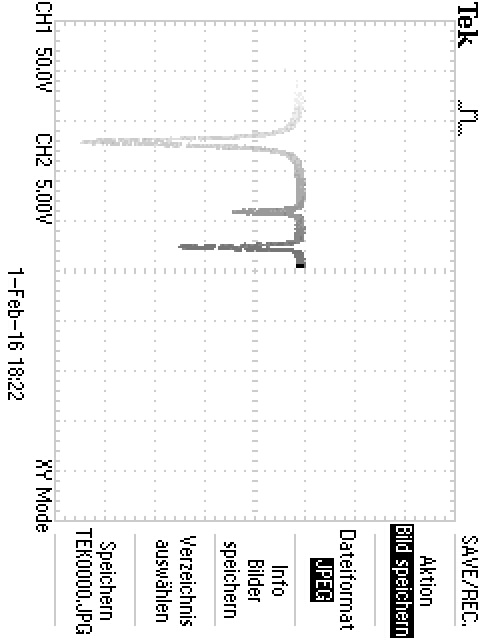
\includegraphics[scale=1,angle=90]{../Grafiken/Signalbild_RF100kHz.jpg}
\caption{Typisches Signalbild des durchgeführten Versuchs, aufgenommen bei einer Frequenz von \SI{100}{\kilo\hertz}. 
	Die Achsen sind Proportional zum anliegenden Magnetfeld ($x$) und der Transparenz des Rubidiumdampfes ($y$). 
	Zusehen sind die Minima für den Nulldurchgang des Magnetfeldes und die Resonanzstellen für die beiden 
	Rubidium-Isotope.\label{fig:signalbild_rf100khz}}
\end{figure}
\FloatBarrier


Die eingestellten Spulenstromstärken der Sweep-Spule und der Horizontalfeld-Spule sind
in \cref{tab:resonanzstellen} in Abhängigkeit der eingestellten Frequenz für die Resonanzstellen
beider Isotope angegeben. Das Gesamtmagnetfeld in horizontaler Richtung, welches aus
den Stromstärken und den gegebenen Abmessungen der Spulen \cref{tab:Apparatur} mit \cref{eq:helmholz_magnetfeld} 
berechnet wurde ist ebenfalls angegeben. Die berechneten Magnetfeld für beide Isotope sind in \cref{fig:resonanzstellen} gegen die jeweiligen
Frequenzen aufgetragen.

\begin{table}[!h]
	\centering
	\begin{adjustbox}{width=\textwidth}
	\begin{tabular}{ccccccc}
		\toprule
		Frequenz & Stromstärke & Stromstärke & Magnetfeld & Stromstärke & Stromstärke & Magnetfeld\\
		$f$/\si{\kilo\hertz} & $I_{1,\mathrm{S}}$/\si{\milli\ampere} & $I_{1,\mathrm{H}}$/\si{\milli\ampere} & $B_{1}$/\si{\milli\tesla} & $I_{2,\mathrm{S}}$/\si{\milli\ampere} & $I_{2,\mathrm{H}}$/\si{\milli\ampere} & $B_{2}$/\si{\micro\tesla}\\
\midrule
		\num{100} & \num{561(1)} & \num{0(3)} & \num{0.034(3)} & \num{680(1)} & \num{0(3)} & \num{41(3)}\\
		\num{200} & \num{579(1)} & \num{15(3)} & \num{0.048(3)} & \num{814(1)} & \num{15(3)} & \num{62(3)}\\
		\num{300} & \num{281(1)} & \num{51(3)} & \num{0.062(3)} & \num{639(1)} & \num{51(3)} & \num{83(3)}\\
		\num{400} & \num{174(1)} & \num{75(3)} & \num{0.076(3)} & \num{649(1)} & \num{75(3)} & \num{104(3)}\\
		\num{500} & \num{199(1)} & \num{90(3)} & \num{0.091(3)} & \num{787(1)} & \num{90(3)} & \num{126(3)}\\
		\num{600} & \num{130(1)} & \num{111(3)} & \num{0.105(3)} & \num{839(1)} & \num{111(3)} & \num{147(3)}\\
		\num{700} & \num{237(1)} & \num{120(3)} & \num{0.120(3)} & \num{671(1)} & \num{150(3)} & \num{172(3)}\\
		\num{800} & \num{401(1)} & \num{126(3)} & \num{0.135(3)} & \num{615(1)} & \num{177(3)} & \num{192(3)}\\
		\num{900} & \num{438(1)} & \num{138(3)} & \num{0.147(3)} & \num{753(1)} & \num{192(3)} & \num{213(3)}\\
		\num{1000} & \num{650(1)} & \num{141(3)} & \num{0.163(3)} & \num{836(1)} & \num{210(3)} & \num{234(3)}\\
		\bottomrule
	\end{tabular}
\end{adjustbox}
	\caption{In Abhängigkeit der eingestellten Frequenz aufgenommenen Stromstärken durch die beiden horizontalen Spulen.
               Die Messwerte der Sweep-Spule sind dabei mit (S) und die der Horizontal-Feld-Spule mit (H) gekennzeichnet.
               Aufgenommen wurden die Stromstärken an den Resonanzstellen für beide Isotope (1) und (2). Mit den
               gegebenen Maßen der Spulen wurde das horizontale Gesamtmagnetfeld aus den Stromstärken bestimmt. \label{tab:resonanzstellen}}
            
\end{table}


\FloatBarrier
\begin{figure}[!h]
\centering
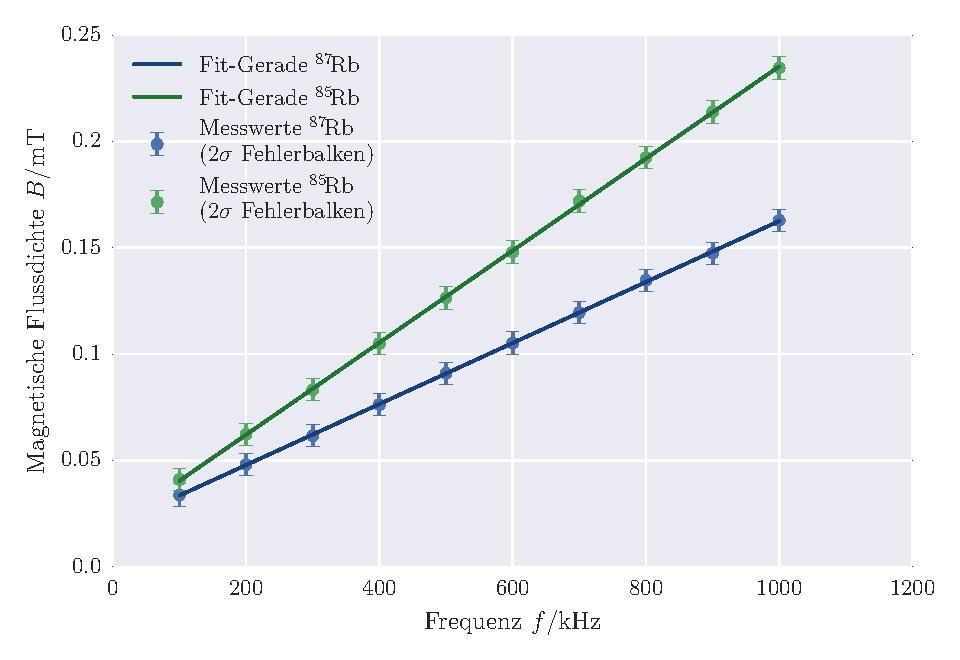
\includegraphics[scale=1]{../Grafiken/Resonanzstellen.pdf}
\caption{Darstellung der berechneten Magnetfelder für beide Isotope in Abhängigkeit der 
	jeweils eingestellten Frequenz. Die Fehlerbalken der Messwerte wurden verdoppelt um sichtbar zu sein.
	Neben den Messwerten sind auch die Ausgleichs-Geraden für beide Isotope dargestellt. \label{fig:resonanzstellen}}
\end{figure}
\FloatBarrier

Die Ausgleichsgraden sind Funktionen der Form
\begin{empheq}{equation}
	B(f) = a\cdot f + b
\end{empheq}
und die entsprechenden Parameter für beide Geraden ergeben sich zu:

\addtocounter{equation}{-1}
\begin{subequations}
	\begin{empheq}{alignat=4}
		a_{1} &=& a =  \SI{1.434(5)e-10}{\tesla\per\hertz}
\qquad
		a_{2} &=& a =  \SI{2.164(9)e-13}{\tesla\per\hertz}
 \\
		b_{1} &=&  \SI{1.92(3)e-05}{\tesla}
\qquad
		b_{2} &=& b =  \SI{1.88(5)e-05}{\tesla}

	\end{empheq}
\end{subequations}

Die theoretische Funktion dieser Geraden entspricht \cref{eq:gerade_magnetfeld_frequenz}. 
Da der Versuchsaufbau parallel respektive antiparallel zum Erdmagnetfeld ausgerichtet wurde, führt 
dieses zu einem Verschiebung entlang der $y$-Achse. Die theoretische Gerade besitzt eine $y$-Achsenabschnitt bei
Null, sodass daraus geschlossen werden, dass die berechneten Parameter $b_i$ der horizontalen Komponente 
Erdmagnetfeld entsprechen. Einen Mittlung der beiden Werte ergibt
\begin{empheq}{equation}
	B_{\mathrm{Erde},\mathrm{hor}} =  \num{1.90(3)e-05}
.
\end{empheq}

Die Steigung der Geraden ist inversproportional zum gesuchten Lande-Faktor $g_{F}$ der beiden Isotope.
Durch Division des konstanten Ausdrucks $\tfrac{h}{\mu_{\mathrm{B}}}$ durch die bestimmten Steigungen $a_{i}$
ergibt sich $g_{F}$ für jedes der Isotope zu
\begin{empheq}{align}
	g_{F,1} &= g_{{}^{87}\!\mathrm{Rb}} =  \num{0.498(2)}
\\
	g_{F,2} &= g_{{}^{85}\!\mathrm{Rb}} =  \num{0.330(1)}

\end{empheq}  

Mit der Kenntnis der Lande-Faktors kann der Kernspin $I$ er beiden Isotope aus \cref{eq:lande_faktor_gf}
bestimmte werden. Für die Berechnung werden zusätzlich der Lande-Faktor des Elektrons $g_{J}$ benötigt.
Dieser lässt sich unter Kenntnis der Quantenzahlen $S$, $L$ und $J$ aus Gleichung \cref{eq:lande_faktor_gj}
bestimmen. Für die Quantenzahlen ergeben sich für diesen Versuch die folgenden Werte.
\begin{empheq}{equation}
	S = \frac{1}{2},\quad L = 0,\quad J = \frac{1}{2},\quad F = I + J
\end{empheq} 
Für $F$ kommt nur der höchst mögliche Wert in Frage, da nur für das Niveau mit dem höchst möglichen $m_F$
kein Übergang mit $\Delta m_{f}$ mehr möglich ist. Einsetzen in \cref{eq:lande_faktor_gf} liefert für die 
Relation

\begin{empheq}{equation}
	I = \frac{1}{2}\del{\frac{g_J}{g_F}-1}
\end{empheq}

für den Kernspin. Die Kernspins der beiden Isotope ergeben sich damit zu
\begin{empheq}{align}
	I_{1} &= I_{{}^{87}\!\mathrm{Rb}} =  \num{1.509(8)}
\\
	I_{2} &= I_{{}^{85}\!\mathrm{Rb}} =  \num{2.53(1)}

\end{empheq}

Ein Vergleich mit den Literatur-Werten für die Kernspins der Rubidium-Isotope \\$I_{\mathrm{Rb85},\mathrm{lit}} = \sfrac{5}{2}$ und $I_{\mathrm{Rb87},\mathrm{lit}} = \sfrac{3}{2}$ lieferte die Zuordung der untersuchten Isotope
\begin{empheq}{equation}
I_{1} = I_{\mathrm{Rb87}},\quad I_{2} = I_{\mathrm{Rb85}}.
\notag
\end{empheq} 

Die Anteile der beiden Isotope $P_{\mathrm{Rb85}}$ und $P_{\mathrm{Rb87}}$ am gesamten können aus dem 
Verhältnis der Größen der beiden Minima in \cref{fig:signalbild_rf100khz} und der Bedingung  
$P_{\mathrm{Rb85}} + P_{\mathrm{Rb87}} = 1$ berechnet werden.
Durch Ausmessen der Pixel beider Minima ergibt sich das Verhältnis der Größen zu
\begin{empheq}{equation}
	R =  \num{0.57(2)}
.
\end{empheq}
Dieses Verhältnis $R$ entspricht dem Verhältnis $\tfrac{P_{\mathrm{Rb87}}}{P_{\mathrm{Rb85}}}$ woraus,
\begin{empheq}{align}
P_{\mathrm{Rb87}} &= \frac{R}{1+R} = P_{{}^{87}\!\mathrm{Rb}} =  \SI{36.4(7)}{\percent}
\\
P_{\mathrm{Rb85}} &= 1-P_{\mathrm{Rb87}} =  \SI{63.6(7)}{\percent}

\end{empheq}
folgt.\\


In der zweite Messung wurden durch Modulation der RF-Spannung zunächst exponentiell Ansteigende und anschließend relaxierende Kurven beobachte. In \cref{fig:exponentieller_anstieg_5v_rubidium_87}  und \cref{fig:exponentieller_anstieg_v6_rubidium_85} ist für jedes der Isotope jeweils ein exponentieller 
Anstieg für eine eingestellte Spannung zusammen mit einer entsprechenden Ausgleichskurve dargestellt.  

\FloatBarrier
\begin{figure}[!h]
\centering
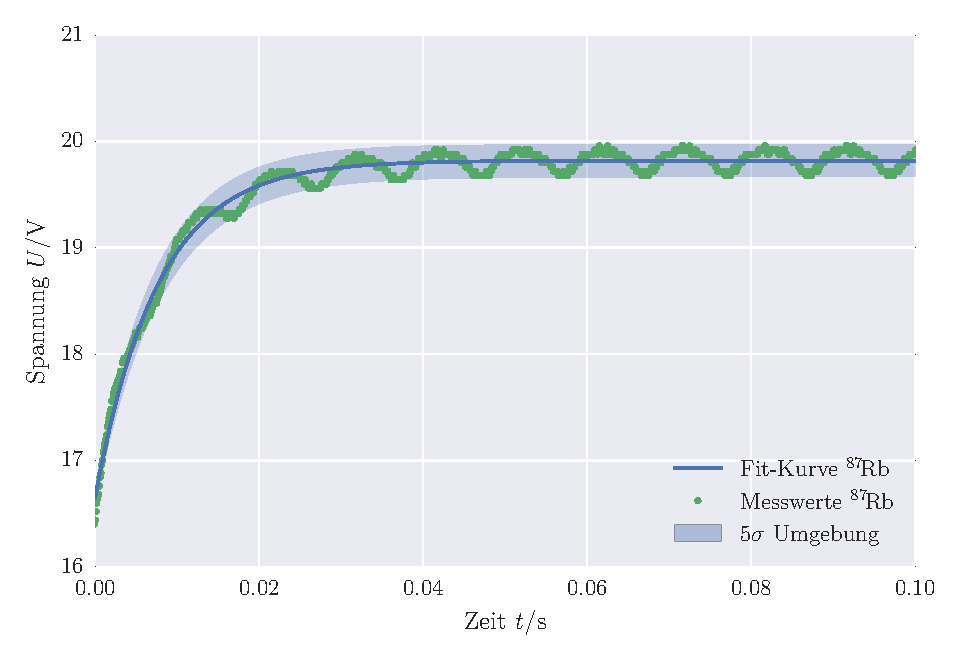
\includegraphics[scale=0.85]{../Grafiken/Exponentieller_Anstieg_5V_Rubidium_87.pdf}
\caption{Darstellung des Exponentiellen Anstiegs der Kurve für ${}^{87}\!$Rb bei einer
	eingestellten RF-Spannung von \SI{5}{\volt}. Zusätzlich ist ein exponentielle Ausgleichskurve 
	der Messwerte dargestellt. \label{fig:exponentieller_anstieg_5v_rubidium_87}}
\end{figure}
\FloatBarrier 
\FloatBarrier
\begin{figure}[!h]
\centering
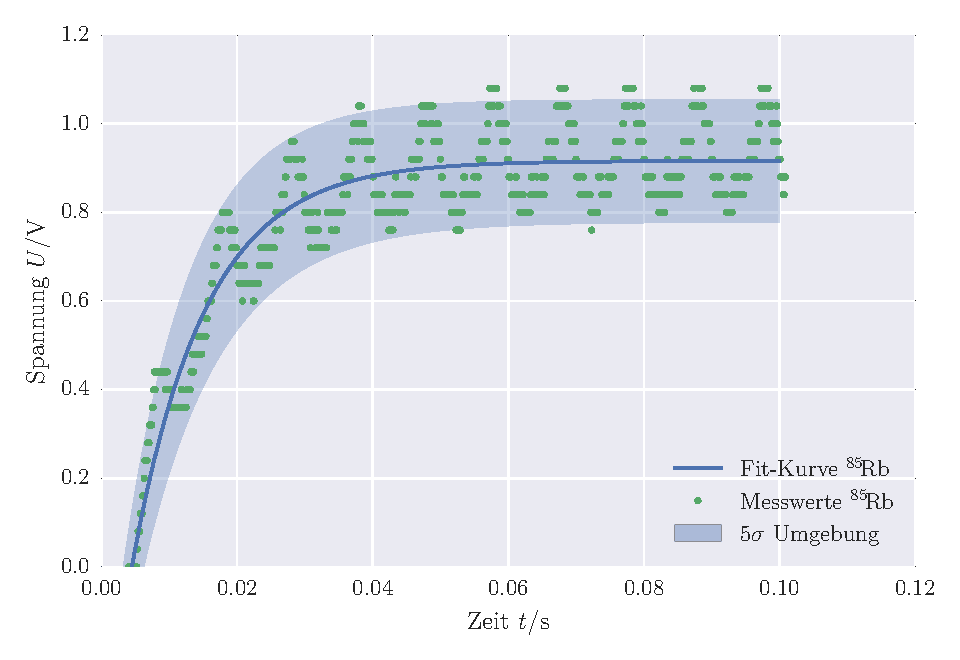
\includegraphics[scale=0.85]{../Grafiken/Exponentieller_Anstieg_V6_Rubidium_85.pdf}
\caption{Darstellung des Exponentiellen Anstiegs der Kurve für ${}^{85}\!$Rb bei einer
	eingestellten RF-Spannung von \SI{6}{\volt}. Zusätzlich ist ein exponentielle Ausgleichskurve 
	der Messwerte dargestellt. \label{fig:exponentieller_anstieg_v6_rubidium_85}}
\end{figure}
\FloatBarrier

Die abgebildeten Ausgleichskurven haben die Form
\begin{empheq}{equation}
	U(t) = a\cdot\del{1-\exp(-b\cdot t)} + c
\end{empheq}

Die Parameter der beiden Ausgleichskurven ergeben sich zu:

\addtocounter{equation}{-1}
\begin{subequations}
	\begin{empheq}{alignat=4}
	a_{\mathrm{Rb87}} &=&  \SI{3.16(2)}{\volt}
\qquad
	a_{\mathrm{Rb85}} &=&  \SI{1.39(1)}{\volt}
 \\
	b_{\mathrm{Rb87}} &=&  \SI{131(1)}{\second}
\qquad 
	b_{\mathrm{Rb85}} &=&  \SI{93(2)}{\second}
\\
	c_{\mathrm{Rb87}} &=&  \SI{16.66(2)}{\volt}
\qquad
	c_{\mathrm{Rb85}} &=&  \SI{-0.47(1)}{\volt}

	\end{empheq}
\end{subequations}

Für die Relaxationen wurden in Abhängigkeit der RF-Spannung die Periodendauer der 
dargestellten gedämpften Schwingung bestimmt. Die dafür aufgenommenen Messwerte,
die Zeitdifferenz und Anzahl der Perioden sind in \cref{tab:periodendauern} für beide 
Isotope angegeben.  

\begin{table}[!h]
	\centering
	\begin{adjustbox}{width=\textwidth}
	\begin{tabular}{ccccccc}
		\toprule
		Spannung & Zeitdifferenz & \# Perioden & Periodendauer & Zeitdifferenz & \# Perioden & Periodendauer\\
		$U$/\si{\volt} & $\Delta t_{1}$/\si{\second} & $N_{1}$ & $T_{1}$/\si{\second} & $\Delta t_{2}$/\si{\second} & $N_{2}$ & $T_{2}$/\si{\second}\\
\midrule
		\num{1} & \num{9.0(1)} & \num{3} & \num{3.00(3)} & \num{1.0(1)} & \num{1} & \num{1.0(1)}\\
		\num{2} & \num{6.4(1)} & \num{4} & \num{1.60(3)} & \num{2.5(1)} & \num{2} & \num{1.26(5)}\\
		\num{3} & \num{6.4(1)} & \num{6} & \num{1.07(2)} & \num{4.3(1)} & \num{4} & \num{1.07(3)}\\
		\num{4} & \num{5.0(1)} & \num{7} & \num{0.71(1)} & \num{2.0(1)} & \num{3} & \num{0.68(3)}\\
		\num{5} & \num{5.2(1)} & \num{8} & \num{0.65(1)} & \num{4.5(1)} & \num{7} & \num{0.65(1)}\\
		\num{6} & \num{3.2(1)} & \num{6} & \num{0.54(2)} & \num{4.4(1)} & \num{9} & \num{0.49(1)}\\
		\num{7} & \num{2.3(1)} & \num{8} & \num{0.28(1)} & \num{4.6(1)} & \num{12} & \num{0.387(8)}\\
		\num{8} & \num{2.2(1)} & \num{8} & \num{0.27(1)} & \num{4.6(1)} & \num{13} & \num{0.351(8)}\\
		\num{9} & \num{2.2(1)} & \num{8} & \num{0.27(1)} & \num{3.1(1)} & \num{10} & \num{0.31(1)}\\
		\num{10} & \num{2.1(1)} & \num{8} & \num{0.27(1)} & \num{3.1(1)} & \num{11} & \num{0.280(9)}\\
		\bottomrule
	\end{tabular}
\end{adjustbox}
	\caption{In Abhängigkeit der eingestellten Spannung aufgenommene Zeitdifferenzen für die jeweilige Anzahl an Perioden.
               Durchgeführt wurde die Messung an den Resonanzstellen beider Isotope bei einer Frequenz von \SI{100}{\kilo\hertz}.
               Aus den aufgenommenen Messwerten wurden die Periodendauern der Relaxtion bestimmt. \label{tab:periodendauern}}
\end{table}


Die bestimmten Periodendauern sind in \cref{fig:transienteneffekt_rubidium_87} und 
\cref{fig:transienteneffekt_rubidium_85} gegen die RF-Spannung aufgetragen dargestellt.
Zusätzlich zu den Messwerten sind noch die hyperbolischen Ausgleichsgeraden abgebildet.

\FloatBarrier
\begin{figure}[!h]
\centering
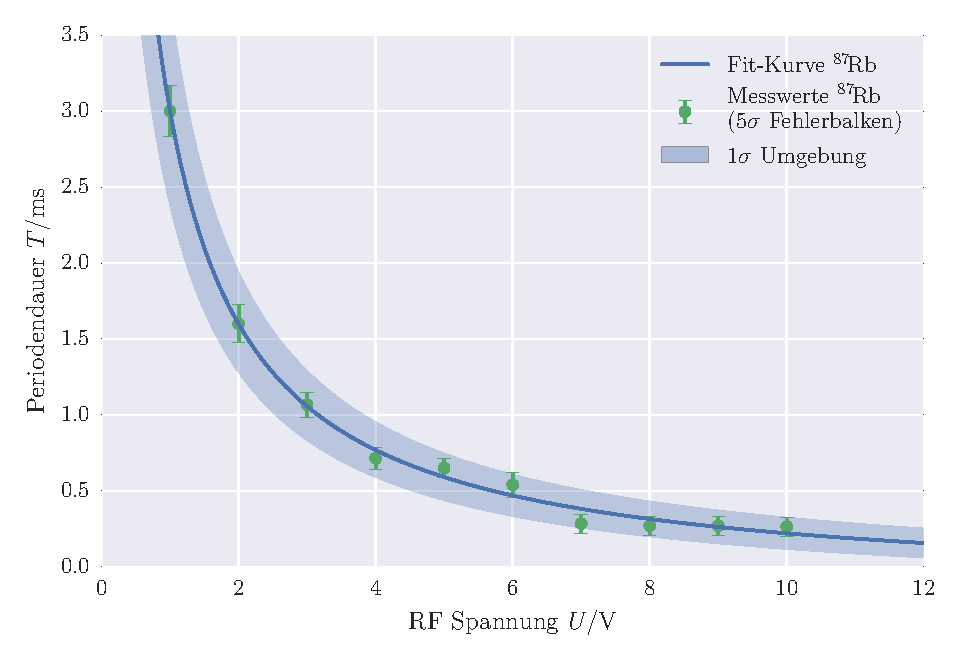
\includegraphics[scale=.85]{../Grafiken/Transienteneffekt_Rubidium_87.pdf}
\caption{In Abhängigkeit der RF-Spannung dargestellte Periodendauern der Relaxation
	für das Isotop ${}^{87}\!$Rb. Die Fehlerbalken der Messwerte wurden verfünffacht, 
	um sichtbar zu sein. Zusätzlich ist die hyperbolische Ausgleichskurve für die Messwerte
	dargestellt. \label{fig:transienteneffekt_rubidium_87}}
\end{figure}
\FloatBarrier 

\FloatBarrier
\begin{figure}[!h]
\centering
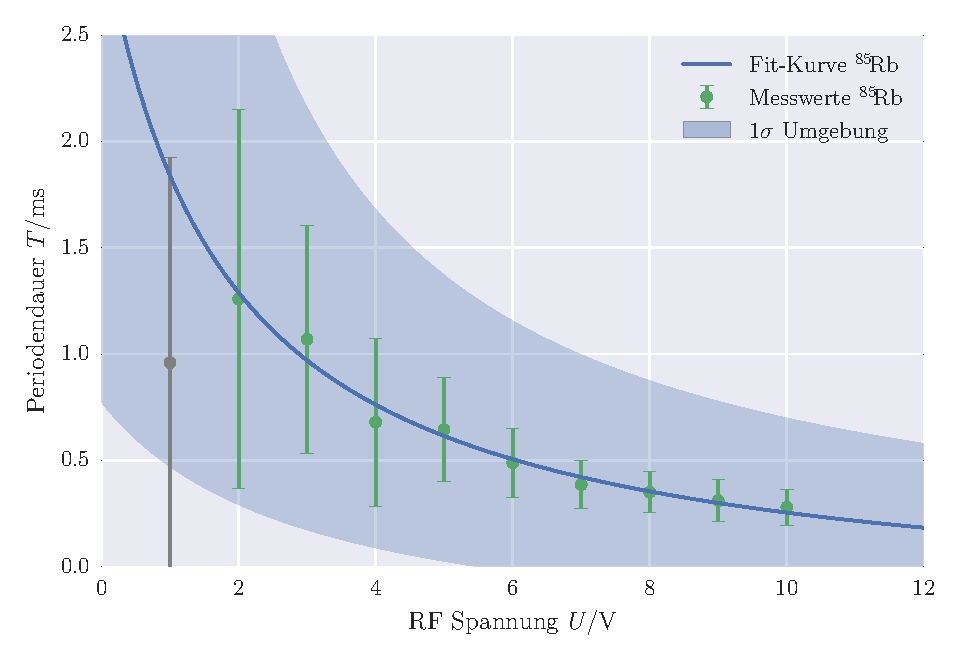
\includegraphics[scale=.8]{../Grafiken/Transienteneffekt_Rubidium_85.pdf}
\caption{In Abhängigkeit der RF-Spannung dargestellte Periodendauern der Relaxation
	für das Isotop ${}^{85}\!$Rb. Die Fehlerbalken der Messwerte wurden verfünffacht, 
	um sichtbar zu sein. Zusätzlich ist die hyperbolische Ausgleichskurve für die Messwerte
	dargestellt. Bei dem abgebildeten Fehlerbereich der Ausgleichskurve handelt es sich nur 
	um einen Bereich mit $\sfrac{1}{50}$ der eigentlichen Größe. Dieser große Fehler ist durch 
	den ersten Messwert bedingt. \label{fig:transienteneffekt_rubidium_85}}
\end{figure}
\FloatBarrier

Für die Ausgleichskurve wurde eine Funktion der Form
\begin{empheq}{equation}
	T(U) = a + \frac{b}{U-c}
\end{empheq} 
verwendet.

Die Parameter für die beiden dargestellten Ausgleichskurven ergeben sich zu:
\addtocounter{equation}{-1}
\begin{subequations}
	\begin{empheq}{alignat=4}
	a_{\mathrm{Rb87}} &=&  \SI{-0.00017(6)}{\second}
\qquad
	a_{\mathrm{Rb85}} &=& a_{{}^{85}\!\mathrm{Rb}} =  \SI{-0.002(6)}{\second}
 \\
	b_{\mathrm{Rb87}} &=&  \SI{0.0040(4)}{\volt\second}
\qquad 
	b_{\mathrm{Rb85}} &=&  \SI{0.1(3)}{\volt\second}
\\
	c_{\mathrm{Rb87}} &=&  \SI{-0.3(1)}{\volt}
\qquad
	c_{\mathrm{Rb85}} &=& c_{{}^{85}\!\mathrm{Rb}} =  \SI{-2.4(5.3)e+01}{\volt}

	\end{empheq}
\end{subequations}


Der Fehlerbereich der Ausgleichskurve für die Messwerte des Isotops ${}^{85}\!$Rb
zeigt sehr große Ungenauigkeiten der Ausgleichskurve. Dies Beobachtung wird auch 
durch die Fehler der Parameter selbst bestätigt. Der Fehler jedes Parameters ist
dabei größer als der bestimmte Parameter selbst. 
Der Grund für diese großen Ungenauigkeiten lässt sich im Verglich mit der anderen 
Ausgleichskurve oder mit einer allgemeinen hyperbolischen Funktion ausfindig machen.
Der Messwert $T(\SI{1}{\volt})$ liegt unter dem $T(\SI{2}{\volt})$, obwohl dieser
wesentlich größer sein müsste, um einen hyperbolischen Verlauf der Messwerte 
darzustellen. Diese Vermutung lässt sich bestätigen indem eine weiterer Ausgleichskurve
an die Messwerte angelegt wird, diesmal wird jedoch der Messwert $T(\SI{1}{\volt})$
nicht berücksichtigt. Die sich so ergebene Ausgleichskurve ist in \cref{fig:transienteneffekt_ausgelassen_rubidium_85} dargestellt.

\FloatBarrier
\begin{figure}[!h]
\centering
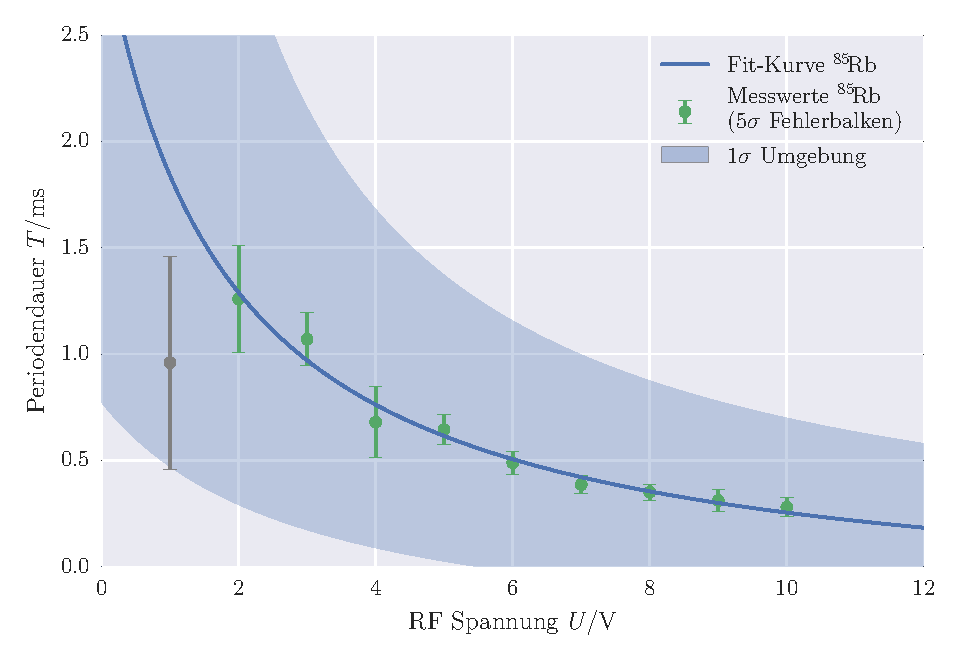
\includegraphics[scale=.85]{../Grafiken/Transienteneffekt_ausgelassen_Rubidium_85.pdf}
\caption{In Abhängigkeit der RF-Spannung dargestellte Periodendauern der Relaxation
	für das Isotop ${}^{85}\!$Rb. Die Fehlerbalken der Messwerte wurden verfünffacht, 
	um sichtbar zu sein. Zusätzlich ist die hyperbolische Ausgleichskurve für die Messwerte
	dargestellt, wobei der grau dargestellte Messwert ausgelassen wurde. 
	\label{fig:transienteneffekt_ausgelassen_rubidium_85}}
\end{figure}
\FloatBarrier

Die Parameter der dritten Ausgleichskurve ergeben sich zu:
\addtocounter{equation}{-1}
\begin{subequations}
	\begin{empheq}{align}
	a^{\prime}_{\mathrm{Rb85}} &= a^{\prime}_{{}^{85}\!\mathrm{Rb}} =  \SI{-0.0002(2)}{\second}
 \\
	b^{\prime}_{\mathrm{Rb85}} &= b^{\prime}_{{}^{85}\!\mathrm{Rb}} =  \SI{0.006(2)}{\volt\second}
\\
	c^{\prime}_{\mathrm{Rb85}} &= c^{\prime}_{{}^{85}\!\mathrm{Rb}} =  \SI{-1.8(1.1)}{\volt}

	\end{empheq}
\end{subequations}

Auch an den Parametern und dem Fehlerbereich dieser Ausgleichskurve sind größere Ungenauigkeiten 
zu erkennen als bei der Ausgleichskurve für ${}^{87}\!$Rb. Diese sind jedoch wesentlich geringer 
als die vorherigen Ungenauigkeiten.

Der Quotient der Parameter $b_{i}$ ergibt für beide Ausgleichskurven einzeln:
\begin{empheq}{align}
	r &= \frac{b_{\mathrm{Rb85}}}{	b_{\mathrm{Rb87}}} =  \num{23(85)}
\\
	r^{\prime} &= \frac{b^{\prime}_{\mathrm{Rb85}}}{b_{\mathrm{Rb87}}} = \num{1.4(6)}

\end{empheq} 
  
